\documentclass{beamer}
\usepackage{../common_slides}
\usepackage{tikz}
\usepackage{tikz-qtree}
\usepackage{pdfpages}

\usetikzlibrary{bayesnet,matrix}
% \usepackage{enumitem}

\title{Sequence Models 2}
\date{}
\author{CS 287}

\def\Lattice{
    \matrix (network)
    [matrix of nodes,
    nodes in empty cells,
    ampersand replacement=\&,
    column sep={1cm},
    row sep={0.1cm},
    nodes={outer sep=0pt,circle,minimum size=0.5cm, minimum width=1.3cm,draw, rectangle} ]
    {
     O \& O \& O \& O \& O\\
     I-PER \& I-PER \& I-PER \& I-PER \& I-PER \\ 
     I-ORG \& I-ORG \& I-ORG \& I-ORG \& I-ORG \\ 
     I-LOC \& I-LOC \& I-LOC \& I-LOC \& I-LOC \\ 
     |[draw=none]| \\
     |[draw=none]| Mayor \& |[draw=none]| DeBlasio \& |[draw=none]| from \& |[draw=none]| New  \& |[draw=none]| York  \\  
};
}

\begin{document}

\begin{frame}
  \titlepage
\end{frame}

\begin{frame}{Review: NER Tagging}
  \begin{description} \itemsep 20pt
  \item[B-TYPE] Stop current mention and begin new mention
    \air 
  \item[I-TYPE] Continue adding to current mention
  \item[O ] Not part of a mention.
  \end{description}
  
  
  \textbf{Example:} \air

  \texttt{[PER \alert{George Bush} ]  [LOC \structure{U.S.} ] president is traveling to [LOC \alert{Baghdad} ] .  } 
\end{frame}


\begin{frame}{Review: Hidden Markov Model}
\begin{center}  
  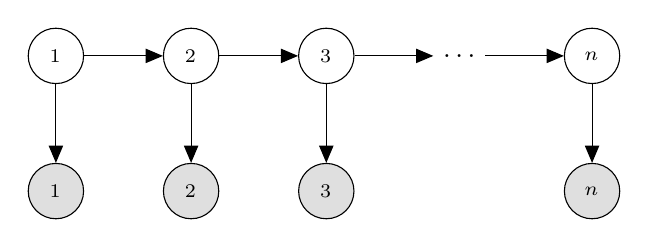
\begin{tikzpicture}
    \node (Ea) [obs] {$\boldx_1$}; 
    \node (Xa) [latent,above =of Ea] {$\boldy_1$}; 

    \node (Eb) [obs, right = of Ea ] {$\boldx_2$}; 
    \node (Xb) [latent,above =of Eb] {$\boldy_2$}; 

    \node (Ec) [obs, right = of Eb] {$\boldx_3$}; 
    \node (Xc) [latent,above =of Ec] {$\boldy_3$}; 
    \node (Xd) [right =of Xc] {$\ldots$}; 
    \node (Xe) [latent,right =of Xd] {$\boldy_n$}; 
    \node (Ee) [obs,below =of Xe] {$\boldx_n$}; 

    \edge {Xa} {Xb} ; %
    \edge {Xb} {Xc} ; %
    \edge {Xa} {Ea} ; %
    \edge {Xb} {Eb} ; %
    \edge {Xc} {Ec} ; %
    \edge {Xc} {Xd} ; %
    \edge {Xd} {Xe} ; %
    \edge {Xe} {Ee} ; %
  \end{tikzpicture}
\end{center}  
\end{frame}


\begin{frame}{Review: Hidden Markov Model}
  Hidden Markov model requires two distributions,
  \begin{itemize}
  \item Transition distribution 
    \[p(\boldy_i | \boldy_{i-1}; \theta)\]
  \item Emission distribution
    \[ p(\boldx_i | \boldy_i ; \theta)\] 
  \end{itemize}


  \begin{itemize}
  \item How many total parameters?
  \end{itemize}
\end{frame}

\begin{frame}{Structured Classification with HMM}

  \begin{itemize}
  \item Interested in find the most-likely $\boldy$ conditioned 
  on input $\boldx$
  \air 

  \item As with naive Bayes, can use joint instead.
  \end{itemize}
 
  \begin{eqnarray*}
     \argmax_{c_{1:n}} p(\boldy_{1:n} = c_{1:n}|  \boldx_{1:n}) &=& \argmax_{c_{1:n}} \log p(\boldy_{1:n} = c_{1:n},  \boldx_{1:n})    \\
    &=& \argmax_{c_{1:n}} \sum_{i=1}^n \log p(\boldy_i | \boldy_{i-1}) + \log p(\boldx_i | \boldy_i )
  \end{eqnarray*}

\end{frame}



\begin{frame}{Review: Maximum Entropy Markov Model}
  MEMM estimates only a transition distribution,
  \begin{itemize}
  \item Transition distribution (also conditioned on input)
    \[p(\boldy_i | \boldy_{i-1}=\delta(c_{i-1}), \boldx_1, \ldots, \boldx_n) = \softmax(feat(\boldx, c_{i-1}) \boldW + \boldb) \]

  \item $feat$;  combination of the input and the previous $c_{i-1}$   
  \end{itemize}
  % \begin{itemize}
  % \item How many total parameters?
  % \end{itemize}
\end{frame}


\begin{frame}{Structured Classification with MEMM}

  \begin{itemize}
  \item Interested in find the most-likely $\boldy$ conditioned 
  on input $\boldx$
  \end{itemize}
 
  \begin{eqnarray*}
     \argmax_{c_{1:n}} p(\boldy_{1:n} = c_{1:n}|  \boldx_{1:n}) &=& \argmax_{c_{1:n}} \log p(\boldy_{1:n} = c_{1:n}|  \boldx_{1:n})    \\
    &=& \argmax_{c_{1:n}} \sum_{i=1}^n \log p(\boldy_i | \boldy_{i-1}, \boldx)
  \end{eqnarray*}
\end{frame}


\begin{frame}{Markov Models}
  \begin{itemize}
  \item In general, intractable to solve sequence prediction,
 
  \[ \argmax_{c_{1:n}} f(\boldx, c_{1:n}) \] 

  \item Today, focus on (first-order) Markov models,

  \[ f(\boldx, c_{1:n})  = \sum_{i=1}^n \log \hat{\boldy}(c_{i-1})_{c_i}\] 

  \item Can extend these ideas to higher-order models.

  \[ f(\boldx, c_{1:n})  = \sum_{i=1}^n \log \hat{\boldy}(c_{i-2}, c_{i-1})_{c_i}\] 
  \end{itemize}  
  
\end{frame}

\begin{frame}{Quiz: History-Based Models}
  Given this definition of a history-based model, 

  \[ f(\boldx, c_{1:n})  = \sum_{i=1}^n \log \hat{\boldy}(c_{i-1})_{c_i} \] 

  Describe the function $g$ for the following models, 

  \begin{enumerate}
  \item Hidden Markov Model
  \item Maximum-Entropy Markov Model
  \item Bigram Language Model (with no $\boldx$, e.g. best $n$ babble)
  \item NNLM with $\dwin=1$
  \end{enumerate}
\end{frame}


\begin{frame}[allowframebreaks]{Answers}
  \begin{itemize}
  \item HMM

    \begin{eqnarray*}
      \log \hat{\boldy}(c_{i-1})_{c_i} &=& \log p(\boldy_i = \delta(c_{i}) | \boldy_{i-1}=\delta(c_{i-1})) + \log p(\boldx_i| \boldy_i )  \\
                                       &=& \log T_{c_{i-1}, c_i}  + \log E_{x_i, c_i}
    \end{eqnarray*}



  \item MEMM
    \[\log \hat{\boldy}(c_{i-1}) = \log \softmax(feat(\boldx, c_{i-1}) \boldW + \boldb)  \]


  % \item Non-probabilistic
  %   \[\log \hat{\boldy}(c_{i-1}) = \log \exp(feat(\boldx, c_{i-1}) \boldW + \boldb)  \]
  %   \pause 
    

  \item Bigram 
    \[\log \hat{\boldy}(c_{i-1})_{c_i} = \log p(\boldy_i = \delta(c_{i}) | \boldy_{i-1}=\delta(c_{i-1}))  \]

  \item NNLM 
    \[\log \hat{\boldy}(c_{i-1}) = \log \softmax(\tanh(v(c_{i-1}) \boldW^1 + \boldb^1) \boldW^2 + \boldb^2)  \]

  \end{itemize}
\end{frame}

\begin{frame}{Today's Lecture}
  Search for Sequences (Fun with Factoring?)
  \[ f(\boldx, c_{1:n})  = \sum_{i=1}^n \log \hat{\boldy}(c_{i-1})_{c_i} \] 
  
  \begin{itemize}
  \item Greedy Search
    \air 
  \item Beam Search
    \air 
  \item Viterbi Search   
  \end{itemize}

  Structured Perceptron
\end{frame}

\begin{frame}{The Lattice}
    \[ f(\boldx, c_{1:n})  = \sum_{i=1}^n \log \hat{\boldy}(c_{i-1})_{c_i} \] 

    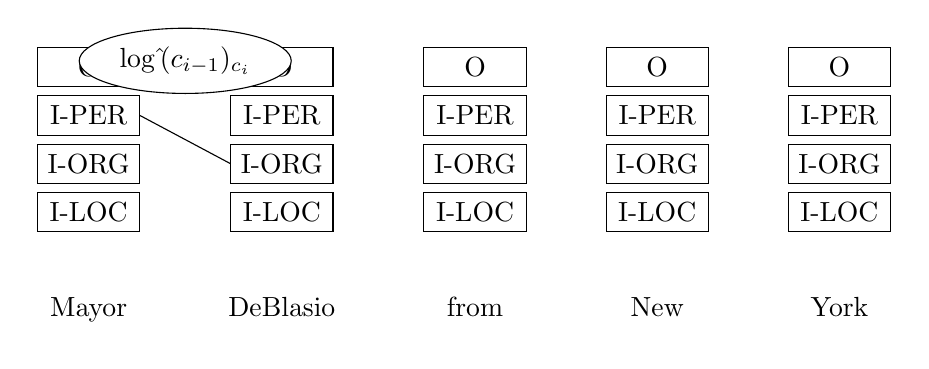
\begin{tikzpicture}
    \Lattice
    \draw<2>[black] (network-2-1.east) -- node[fill=white, yshift=1cm,draw, ellipse] {$\log \hat{\boldy}(c_{i-1})_{c_i}$}  (network-3-2.west);
    \end{tikzpicture}
\end{frame}

\begin{frame}{Exponentially Many Sequences}
  \begin{center}   
  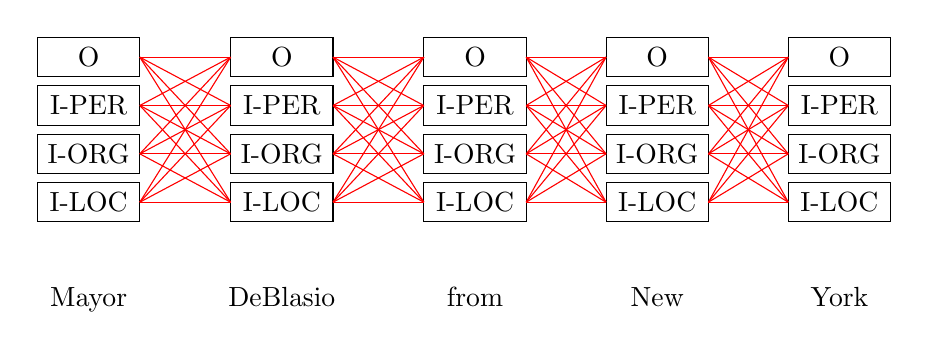
\begin{tikzpicture}
    \Lattice
    \foreach \i in {1,...,4} {
    \foreach \j in {1,...,4} {
    \draw[red] (network-\i-1.east) -- (network-\j-2.west);
    \draw[red] (network-\i-2.east) -- (network-\j-3.west);
    \draw[red] (network-\i-3.east) -- (network-\j-4.west);
    \draw[red] (network-\i-4.east) -- (network-\j-5.west);
    % \draw<8->[blue] (network-\i-1.east) -- (network-\j-2.west);
    % \draw<7->[blue] (network-\i-2.east) -- (network-\j-3.west);
    % \draw<6->[blue] (network-\i-3.east) -- (network-\j-4.west);
    % \draw<5->[blue] (network-\i-4.east) -- (network-\j-5.west);

    } }
  \end{tikzpicture}
  \end{center}  
\end{frame}



\begin{frame}{A Single Sequence}
  \begin{center}
    \[ f(\boldx, c_{1:n})  = \log \hat{\boldy}(c_{1})_{c_2} + \log \hat{\boldy}(c_{2})_{c_3} + \log \hat{\boldy}(c_{3})_{c_4} + \log \hat{\boldy}(c_{4})_{c_5} \]    

  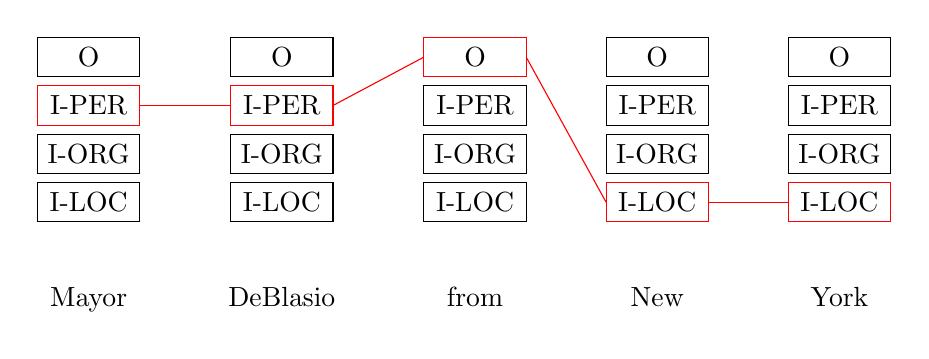
\begin{tikzpicture}
    \Lattice
    \draw[red] (network-2-1.north west) rectangle  (network-2-1.south east);
    \draw[red] (network-2-2.north west) rectangle  (network-2-2.south east);
    \draw[red] (network-1-3.north west) rectangle  (network-1-3.south east);
    \draw[red] (network-4-4.north west) rectangle  (network-4-4.south east);
    \draw[red] (network-4-5.north west) rectangle  (network-4-5.south east);

    \draw[red] (network-2-1.east) --  (network-2-2.west);
    \draw[red] (network-2-2.east) -- (network-1-3.west); 
    \draw[red] (network-1-3.east) -- (network-4-4.west);
    \draw[red] (network-4-4.east) -- (network-4-5.west);
    
  \end{tikzpicture}
  \end{center}
      % |[draw=none]| & |[xshift=1mm]| & |[xshift=-1mm]| \\
\end{frame}

\section{Heuristic Search}

\begin{frame}{Heuristic Search}
  \begin{itemize}
  \item Fast method for finding a solution.

    \air 
  \item Often can be quite effective in practice.
    \air 
  \item Tradeoff: More powerful models/less exact search. 
    
  \end{itemize}
\end{frame}

\begin{frame}[fragile]{Algorithm 1: Greedy Search}
  \begin{center}
    \begin{algorithmic}
      \Procedure{GreedySearch}{} \State{$s = 0$} \Comment{Running score}
      \State{$c \in \mcC^{n+1}$}  \Comment{Sequence}
      \State{$c_0 = \langle s \rangle$} \Comment{Initial Symbol}
      \For{$i = 1$ to $n$ }
      \State{$c_i \gets\displaystyle \argmax_{c'_i} \hat{\boldy}(c_{i-1})_{c'_i}$}
      \State{$s \gets s + \log \hat{\boldy}(c_{i-1})_{c_i}$}
      \EndFor{}
      \State{\Return{$c, s$}}
      \EndProcedure{}
    \end{algorithmic}
  \end{center}
  \pause 

  \begin{itemize}
  \item Time Complexity?
  \item Space Complexity?
  \end{itemize}
\end{frame}


\begin{frame}{Greedy Search}
    \[ f(\boldx, c_{1:n})  = \sum_{i=1}^n \log \hat{\boldy}(c_{i-1})_{c_i} \] 

    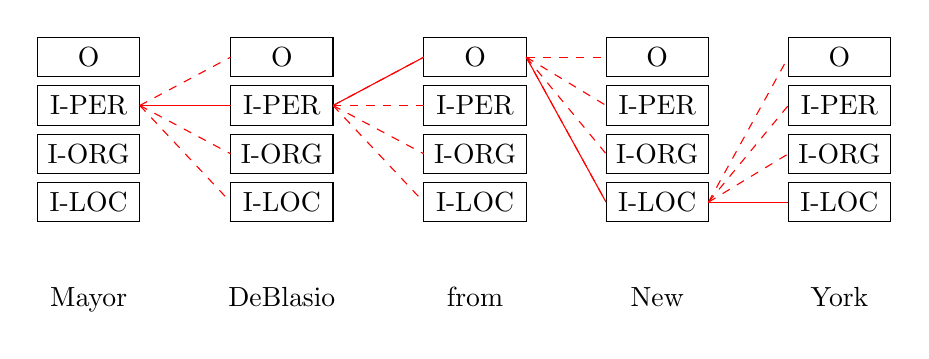
\begin{tikzpicture}
    \Lattice
    \draw<2->[red] (network-2-1.east) --  (network-2-2.west);
    \draw<3->[red] (network-2-2.east) -- (network-1-3.west); 
    \draw<4->[red] (network-1-3.east) -- (network-4-4.west);
    \draw<5->[red] (network-4-4.east) -- (network-4-5.west);

    \foreach \j in {1,...,4} {
    \draw<1>[red,dashed] (network-2-1.east) -- (network-\j-2.west);
    \draw<2>[red,dashed] (network-2-2.east) -- (network-\j-3.west);
    \draw<3>[red,dashed] (network-1-3.east) -- (network-\j-4.west);
    \draw<4>[red,dashed] (network-4-4.east) -- (network-\j-5.west);
    } 

    \end{tikzpicture}
\end{frame}

\begin{frame}{Issues}
  \begin{itemize}
  \item What cases does beam search fail?
    \air
  \item How might we get around these issues without hurting time/space complexity?

  \end{itemize}
\end{frame}

\begin{frame}[fragile]{Algorithm 2: Beam Search}
  \begin{itemize}
  \item Idea: Maintain multiple hypotheses.
    \air
  \item Each step keep $k$ highest scoring.
    \air 
  \item Hypotheses with different histories compete.
  \end{itemize}
\end{frame}


\begin{frame}[fragile]{Algorithm 2: Beam Search}
  
  \begin{center}
    \begin{algorithmic}
      \Procedure{BeamSearch}{$K$} 
      \State{K sequences $c[1], \ldots, c[K]$} 
      \State{$s_k \gets 0, c[k]_0 = \langle s \rangle$ for all $k$} \Comment{Initialize}
      \For{$i = 1$ to $n$ }
      \State{hyps $\gets \{\}$}
      \For{$k = 1$ to $K$ }
      \For{$c_i \in \mcC$ }
      \State{$s' \gets  s_k + \log \hat{\boldy}(c[k]_{i-1})_{c_i} $}
      \State{hyps add $(c[k] + [c_i], s')$}
      \EndFor{}
      \For{$k = 1$ to $K$ }
      \State{$c[k], s_k  \gets$ pop highest score in hyps }
      \EndFor{}
      \EndFor{}
      \EndFor{}
      \State{\Return{$c[1], s_1$}}
      \EndProcedure{}
    \end{algorithmic}
  \end{center}
\end{frame}

\begin{frame}{Questions: Beam Search}
  \begin{itemize}
  \item Space Complexity?

    \air 
  \item Time Complexity?
    \air 

  \item Optimality?
    \air 

  \item Versus $K$ runs of beam search? 
    \air 

  \end{itemize}
\end{frame}




\begin{frame}{Beam Search (K=2)}
    \[ f(\boldx, c_{1:n})  = \sum_{i=1}^n \log \hat{\boldy}(c_{i-1})_{c_i} \] 

    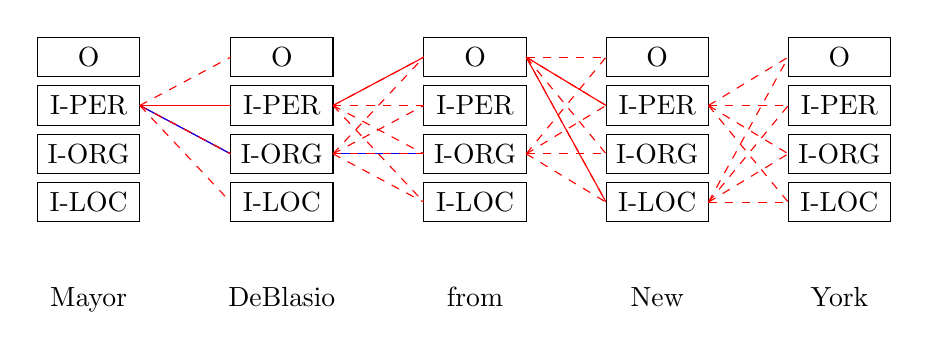
\begin{tikzpicture}
    \Lattice
    \draw<2->[red] (network-2-1.east) --  (network-2-2.west);
    \draw<2-3>[red] (network-2-1.east) --  (network-3-2.west);
    \draw<4>[blue] (network-2-1.east) --  (network-3-2.west);
    \draw<3->[red] (network-2-2.east) -- (network-1-3.west); 
    \draw<3>[red] (network-3-2.east) -- (network-3-3.west); 
    \draw<4>[blue] (network-3-2.east) -- (network-3-3.west); 
    \draw<4->[red] (network-1-3.east) -- (network-4-4.west);
    \draw<4->[red] (network-1-3.east) -- (network-2-4.west);

    \foreach \j in {1,...,4} {
    \draw<1>[red,dashed] (network-2-1.east) -- (network-\j-2.west);
    \draw<2>[red,dashed] (network-2-2.east) -- (network-\j-3.west);
    \draw<2>[red,dashed] (network-3-2.east) -- (network-\j-3.west);
    \draw<3>[red,dashed] (network-1-3.east) -- (network-\j-4.west);
    \draw<3>[red,dashed] (network-3-3.east) -- (network-\j-4.west);
    \draw<4>[red,dashed] (network-4-4.east) -- (network-\j-5.west);
    \draw<4>[red,dashed] (network-2-4.east) -- (network-\j-5.west);
    } 

    \end{tikzpicture}
\end{frame}


\begin{frame}{Beam Search for Markov Models}

  \begin{itemize}
  \item Does this use the Markov property?
    \air 
  \item (How would beam search differ for RNN and HMM?)

  \end{itemize}
\end{frame}

\begin{frame}{Beam Search}
    \[ f(\boldx, c_{1:n})  = \sum_{i=1}^n \log \hat{\boldy}(c_{i-1})_{c_i} \] 

    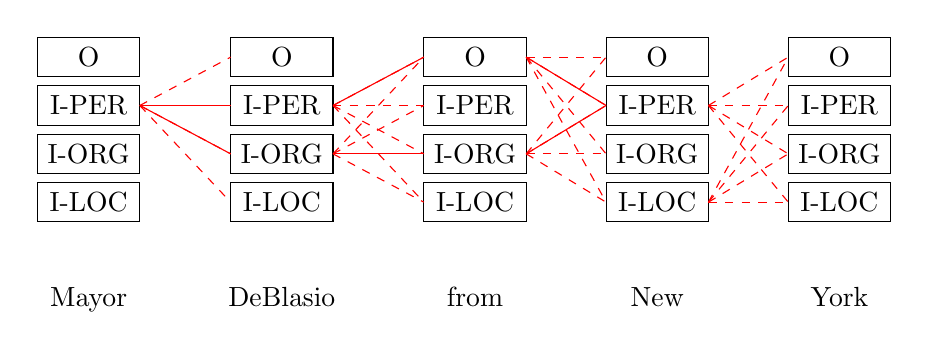
\begin{tikzpicture}
    \Lattice
    \draw<2->[red] (network-2-1.east) --  (network-2-2.west);
    \draw<2->[red] (network-2-1.east) --  (network-3-2.west);
    \draw<3->[red] (network-2-2.east) -- (network-1-3.west); 
    \draw<3->[red] (network-3-2.east) -- (network-3-3.west); 
    \draw<4->[red] (network-1-3.east) -- (network-2-4.west);
    \draw<4->[red] (network-3-3.east) -- (network-2-4.west);

    \foreach \j in {1,...,4} {
    \draw<1>[red,dashed] (network-2-1.east) -- (network-\j-2.west);
    \draw<2>[red,dashed] (network-2-2.east) -- (network-\j-3.west);
    \draw<2>[red,dashed] (network-3-2.east) -- (network-\j-3.west);
    \draw<3>[red,dashed] (network-1-3.east) -- (network-\j-4.west);
    \draw<3>[red,dashed] (network-3-3.east) -- (network-\j-4.west);
    \draw<4>[red,dashed] (network-4-4.east) -- (network-\j-5.west);
    \draw<4>[red,dashed] (network-2-4.east) -- (network-\j-5.west);
    } 

    \end{tikzpicture}
\end{frame}

\begin{frame}[fragile]{Algorithm 2: Beam Search With Recombination}
  \begin{center}
    \begin{algorithmic}
      \Procedure{BeamSearch}{$K$} 
      \State{$c \in \mcC^{K \times n+1}$} 
      \State{$s_k \gets 0, c[k]_0 = \langle s \rangle$ for all $k$}
      \For{$i = 1$ to $n$ }
      \State{hyps $\gets \{\}$}
      \For{$k = 1$ to $K$ }
      \For{$c_i \in \mcC$ }
      \State{$s' \gets  s_k + \log \hat{\boldy}(c[k]_{i-1})_{c_i} $}
      \State{hyps add $(c[k] + c_i, s')$}
      \EndFor{}
      \For{$k = 1$ to $K$ }
      \State{$c[k], s_k  \gets$ pop highest score in hyps \alert{with unique $c_i$} }
      \EndFor{}
      \EndFor{}
      \EndFor{}
      \State{\Return{$c[1], s_1$}}
      \EndProcedure{}
    \end{algorithmic}
  \end{center}
\end{frame}


\begin{frame}{Exact Solutions}
  \begin{itemize}
  \item Greedy search and beam search are approximate (heuristic).
    \air
  \item Neither really exploit Markov assumption.

    \air 

  \item Exact algorithm for sequences known as Viterbi (1967) decoding 
  \end{itemize}
\end{frame}

\section{Viterbi}

\begin{frame}{Dynamic Programming over a Lattice}
  \begin{itemize}
  \item Several different varieties: Viterbi, forward, backward

  \item Recursive Definition:
    \begin{itemize}
    \item Base Case: Start with the score for sequence of length 1.  \air
    \item Inductive Case: Compute all sequences of length $i$ from $i-1$ 
    \end{itemize}
  \end{itemize}

  \begin{center}   
  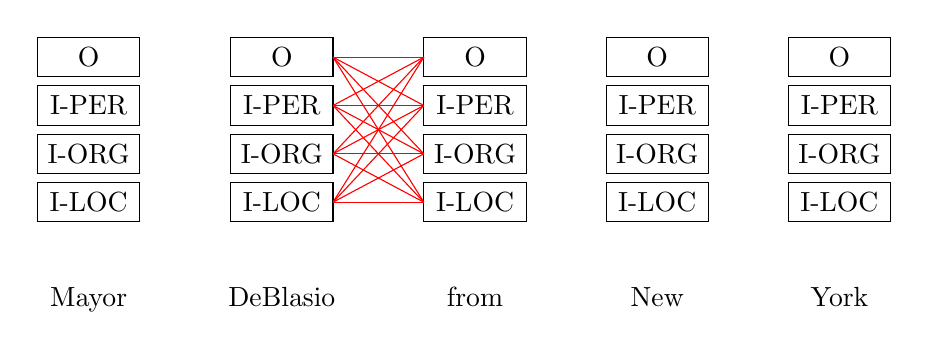
\begin{tikzpicture}
    \Lattice
    \foreach \i in {1,...,4} {
    \foreach \j in {1,...,4} {
    \draw[red] (network-\i-2.east) -- (network-\j-3.west);
    } }
  \end{tikzpicture}
  \end{center}  

\end{frame}

\begin{frame}{Viterbi Algorithm (Simple)}
  \begin{algorithmic}
    \Procedure{Viterbi}{}
    \State{$\pi \in \reals^{ (n+1) \times \mcC}$ initialized to $-\infty$ }
    \State{$\pi[0, \langle s \rangle] = 0$}
    \For{$i = 1$ to $n$ }
    \For{$c_{i} \in \mcC$}
    \State{$\pi[i, c_i] = \max_{c_{i-1}} 
     \pi[i-1, c_{i-1}] + \log \hat{\boldy}(c_{i-1})_{c_i}        
       $}
    \EndFor{}
    \EndFor{}
    \State{\Return{$\max_{c_n\in\mcC} \pi[n, c_n]$}}
    \EndProcedure{}
  \end{algorithmic}
  \begin{itemize}
  \item Time Complexity?
  \item Space Complexity?
  \end{itemize}
\end{frame}

\begin{frame}{The Main Max-Step}
  \begin{center}
  \begin{algorithmic}
    \For{$c_{i} \in \mcC$}
    \State{$\pi[i, c_i] = \max_{c_{i-1}} 
     \pi[i-1, c_{i-1}] + \log \hat{\boldy}(c_{i-1})_{c_i}        
       $}
    \EndFor{}
  \end{algorithmic}
  \air \air
   
  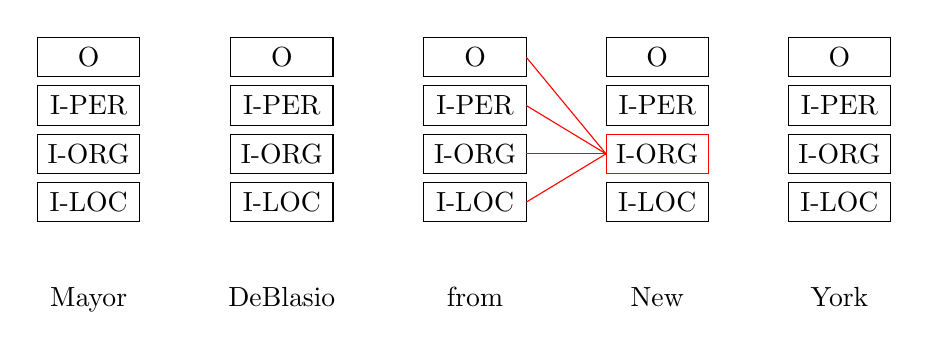
\begin{tikzpicture}
    \Lattice
    \draw[red] (network-3-4.north west) rectangle  (network-3-4.south east);

    \draw[red] (network-1-3.east) -- (network-3-4.west);
    \draw[red] (network-2-3.east) -- (network-3-4.west); 
    \draw[red] (network-3-3.east) -- (network-3-4.west);
    \draw[red] (network-4-3.east) -- (network-3-4.west);
  \end{tikzpicture}
  \end{center}
      % |[draw=none]| & |[xshift=1mm]| & |[xshift=-1mm]| \\
\end{frame}


\begin{frame}{Computation and Ordering}
  \begin{center}
  \begin{algorithmic}
    \For{$c_{i} \in \mcC$}
    \State{$\pi[i, c_i] = \max_{c_{i-1}} 
     \pi[i-1, c_{i-1}] + \log \hat{\boldy}(c_{i-1})_{c_i}        
       $}
    \EndFor{}
  \end{algorithmic}
  \air \air

  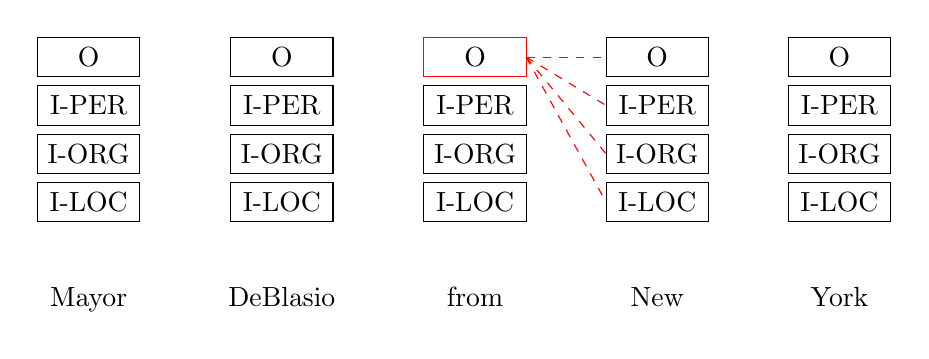
\begin{tikzpicture}
    \Lattice
    \draw[red] (network-1-3.north west) rectangle  (network-1-3.south east);

    \draw[red,dashed] (network-1-3.east) -- (network-1-4.west);
    \draw[red,dashed] (network-1-3.east) -- (network-2-4.west); 
    \draw[red,dashed] (network-1-3.east) -- (network-3-4.west);
    \draw[red,dashed] (network-1-3.east) -- (network-4-4.west);
  \end{tikzpicture}
  \end{center}
      % |[draw=none]| & |[xshift=1mm]| & |[xshift=-1mm]| \\
\end{frame}



\begin{frame}{Viterbi Algorithm with Precompute}
  \begin{algorithmic}
    \Procedure{ViterbiWithPrecompute}{}
    \State{$\pi \in \reals^{n \times \mcC}$ initialized to $-\infty$ }
    \State{$\pi[0, \langle s \rangle] = 0$}
    \For{$i = 1$ to $n$ }
    \For{$c_{i-1} \in \mcC$}
    \State{precompute \alert{$\hat{\boldy}(c_{i-1})$}}
    \For{$c_{i} \in \mcC$}
    \State{$score = \pi[i-1, c_{i-1}] + \log \hat{\boldy}(c_{i-1})_{c_i} $}
    \If{$score > \pi[i, c_i]$}
    \State{$\pi[i, c_i] = score$}
    \EndIf{}
    \EndFor{}
    \EndFor{}
    \EndFor{}
    \State{\Return{$\max_{c_n\in\mcC} \pi[n, c_n]$}}
    \EndProcedure{}
  \end{algorithmic}

\end{frame}





\begin{frame}{Viterbi Algorithm with Backpointers}
  \begin{algorithmic}
    \Procedure{ViterbiWithBP}{}
    \State{$\pi \in \reals^{ n+1 \times \mcC}$ initialized to $-\infty$ }
    \State{\alert{$bp \in \mcC^{n \times \mcC}$} initialized to $\epsilon$ }
    \State{$\pi[0, \langle s \rangle] = 0$}
    \For{$i = 1$ to $n$ }
    \For{$c_{i-1} \in \mcC$}
    \State{compute $\hat{\boldy}(c_{i-1})$}
    \For{$c_{i} \in \mcC$}
    \State{$score = \pi[i-1, c_{i-1}] + \log \hat{\boldy}(c_{i-1})_{c_i} $}
    \If{$score > \pi[i, c_i]$}
    \State{$\pi[i, c_i] = score$}
    \State{\alert{$bp[i, c_i] = c_{i-1}$}}
    \EndIf{}
    \EndFor{}
    \EndFor{}
    \EndFor{}
    \State{\Return{\alert{sequence from $bp$}}}
    \EndProcedure{}
  \end{algorithmic}
\end{frame}

\begin{frame}{Walking Back}
  \begin{center}
    Matrix $ bp $ 
  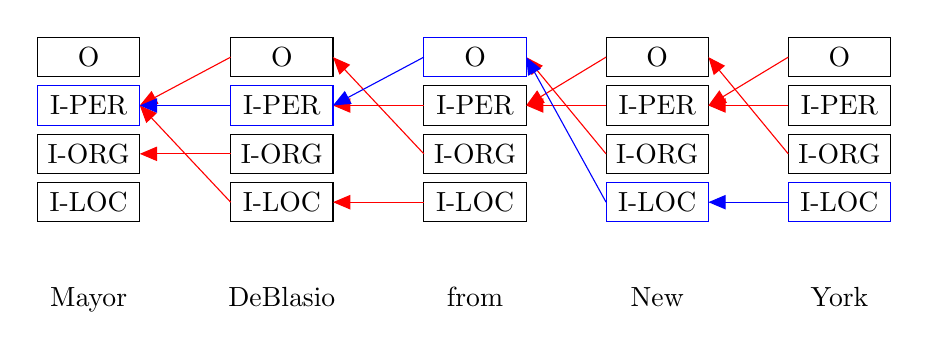
\begin{tikzpicture}
    \Lattice

    \draw[red,<-] (network-2-1.east) --  (network-1-2.west);

    \draw[red,<-] (network-3-1.east) --  (network-3-2.west);
    \draw[red,<-] (network-2-1.east) --  (network-4-2.west);
    \draw[blue,<-] (network-2-1.east) --  (network-2-2.west);


    \draw[red,<-] (network-2-2.east) --  (network-2-3.west);
    \draw[red,<-] (network-1-2.east) --  (network-3-3.west);
    \draw[red,<-] (network-4-2.east) --  (network-4-3.west);
    \draw[blue,<-] (network-2-2.east) --  (network-1-3.west);

    \draw[red,<-] (network-2-3.east) --  (network-1-4.west);
    \draw[red,<-] (network-2-3.east) --  (network-2-4.west);
    \draw[red,<-] (network-1-3.east) --  (network-3-4.west);
    \draw[blue,<-] (network-1-3.east) --  (network-4-4.west);

    \draw[red,<-] (network-2-4.east) --  (network-1-5.west);
    \draw[red,<-] (network-2-4.east) --  (network-2-5.west);
    \draw[red,<-] (network-1-4.east) --  (network-3-5.west);
    \draw[blue,<-] (network-4-4.east) --  (network-4-5.west);

    \draw[blue] (network-2-1.north west) rectangle  (network-2-1.south east);
    \draw[blue] (network-2-2.north west) rectangle  (network-2-2.south east);
    \draw[blue] (network-1-3.north west) rectangle  (network-1-3.south east);
    \draw[blue] (network-4-4.north west) rectangle  (network-4-4.south east);
    \draw[blue] (network-4-5.north west) rectangle  (network-4-5.south east);


    % \draw[red] (network-2-1.east) --  (network-1-2.west);
    % \draw[red] (network-2-1.east) --  (network-2-2.west);
    % \draw[red] (network-3-1.east) --  (network-3-2.west);
    % \draw[red] (network-2-1.east) --  (network-4-2.west);


    
  \end{tikzpicture}
  \end{center}
      % |[draw=none]| & |[xshift=1mm]| & |[xshift=-1mm]| \\
\end{frame}

\begin{frame}{Decoding with MEMM}
  \begin{itemize}
  \item Allows features on previous sequence information.
    \air 
  \item If $|\mcC|$ is reasonable, quite fast to decode.
    \air 

  \item If $|\mcC|$ is large, can use approximations (others coming up as well).
    \air
  \item However, still not trained for sequence prediction.
  \end{itemize}
\end{frame}

\section{Structured Perceptron}

\begin{frame}{Recall: Issues with Multiclass for Sequences }
  \begin{itemize}
  \item Say there are $\mcT$ tags and sequence length is $n$
    \air 

  \item There are $\dout = O(\mcT^n)$ sequences! 
    \air 
  \item Just naively computing the softmax is exponential in length. 
    \air 

  \item Even if you could compute the softmax, $\boldW \in \reals^{\din \times \dout}$ would 
    be impossible to train.
  \end{itemize}
\end{frame}


\begin{frame}{Answers?}
  \begin{itemize}
  \item If we have Markov structure, finding max is fast,
    \[ f(\boldx, c_{1:n})  = \sum_{i=1}^n \log \hat{\boldy}(c_{i-1})_{c_i}\]   
    \air 

  \item Can have local features, with small $\boldW$ (no softmax)
    \[\log \hat{\boldy}(c_{i-1})_{c_i} = feat(\boldx, c_{i-1}) \boldW + \boldb\]
    
    \air 

  \item Can use hinge-loss instead of taking the full softmax. 

    \air 
  \item (Next class, revisit softmax)
  \end{itemize}

\end{frame}

\begin{frame}{Review: Hinge Loss}

  \[{\mathcal{L}(\theta)} = \sum_{i=1}^n L_{hinge}(\boldy,\hat{\boldy}) \] 


  \[ L_{hinge}(\boldy, \hat{\boldy}) =  \max\{0, 1 - (\hat{y}_{c} - \hat{y}_{c'}) \}  \]

  Where 
  \begin{itemize}
  \item   Let $c$ be defined as true class $y_{i, c} = 1$  
    \[c' = \argmax_{i \in \mcC \setminus\{c\}} \hat{y}_i \] 
  \end{itemize}

  \pause

  Minimizing hinge loss is an upper-bound for 0/1. 

  \[ L_{hinge}(\boldy, \hat{\boldy}) \geq L_{0/1}(\boldy, \hat{\boldy})\] 
\end{frame}


\begin{frame}{Simple Structured Hinge}
  \[{\mathcal{L}(\theta)} = \sum_{i=1}^n L_{shinge}(\boldy,\hat{\boldy}) \] 


  \[ L_{shinge}(\boldy, \hat{\boldy}) =  \max\{0, 1 - (f(\boldx, c_{1:n}) - f(\boldx, {c'_{1:n}})) \}  \]

  Where 
  \begin{itemize}
  \item   Let $c_{1:n}$ be defined as true classes $y_{i, c} = 1$  
    \[c'_{1:n} = \argmax_{c' \neq c } f(\boldx, c'_{1:n}) \] 
  \end{itemize}
  
  \begin{itemize}
  \item What do the gradients look like?
  \end{itemize}

\end{frame}


\begin{frame}{Symbolic Gradients}

  \begin{itemize}
  \item   Let $c_{1:n}$ be defined as true sequence
  \item   Let $c'_{1:n}$ be defined as the highest scoring non-true sequence 
    \[c'_{1:n} = \argmax_{c' \neq c} f(\boldx, c'_{1:n}) \]
  \item Partials of $L(y, \hat{y})$

  \[ \frac{\partial L(y,k \hat{y})}{\partial \log \hat{y}_{i,j}} =
      \begin{cases}
         0 & f(\boldx, c_{1:n}) - f(\boldx, {c'_{1:n}} > 1  \\
         1 & j = c'_i \land j \neq c_i \\
         -1 & j = c_i \land j \neq c'_i \\
         0 & o.w. \\ 
      \end{cases}
  \]
  \end{itemize}
  Intuition: If wrong or close to wrong, improve correct and lower closest incorrect positions (when they disagree).
\end{frame}

\begin{frame}{Updates}
  \begin{itemize}
  \item \alert{red} - $c'$ 
  \item \structure{blue} - $c$
  \item black - both
  \end{itemize}
  \air

  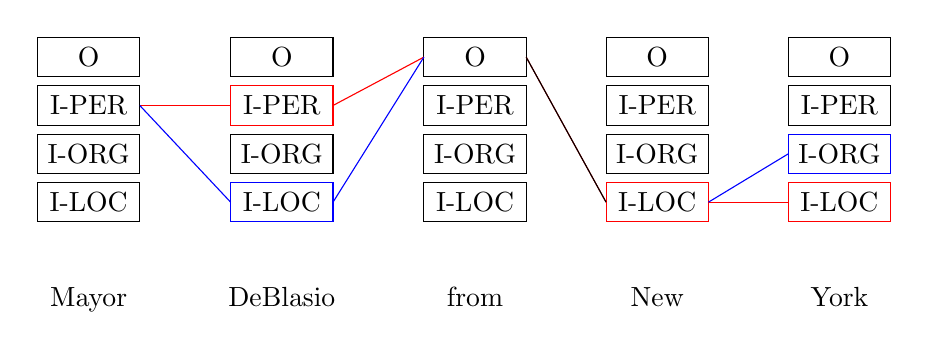
\begin{tikzpicture}
    \Lattice
    \draw[black] (network-2-1.north west) rectangle  (network-2-1.south east);
    \draw[red] (network-2-2.north west) rectangle  (network-2-2.south east);
    \draw[black] (network-1-3.north west) rectangle  (network-1-3.south east);
    \draw[red] (network-4-4.north west) rectangle  (network-4-4.south east);
    \draw[red] (network-4-5.north west) rectangle  (network-4-5.south east);
    \draw[blue] (network-3-5.north west) rectangle  (network-3-5.south east);
    \draw[blue] (network-4-2.north west) rectangle  (network-4-2.south east);

    \draw[red] (network-2-1.east) --  (network-2-2.west);
    \draw[red] (network-2-2.east) -- (network-1-3.west); 
    \draw[red] (network-1-3.east) -- (network-4-4.west);
    \draw[red] (network-4-4.east) -- (network-4-5.west);

    \draw[blue] (network-2-1.east) --  (network-4-2.west);
    \draw[blue] (network-4-2.east) -- (network-1-3.west); 
    \draw[black] (network-1-3.east) -- (network-4-4.west);
    \draw[blue] (network-4-4.east) -- (network-3-5.west);
    
  \end{tikzpicture}
\end{frame}

\begin{frame}{Structured Perceptron}
  Similar method without margin
  \begin{itemize}
  \item   Let $c_{1:n}$ be defined as true sequence
  \item   Let $c'_{1:n}$ be defined as the highest scoring non-true sequence 
    \[c'_{1:n} = \argmax_{c' \neq c } f(\boldx, c'_{1:n}) \] 
  \item Partials of $L(y, \hat{y})$

  \[ \frac{\partial L(y,k \hat{y})}{\partial \log \hat{y}_{i,j}} =
      \begin{cases}
         0 & f(\boldx, c_{1:n}) - f(\boldx, {c'_{1:n}} > 0  \\
         1 & j = c'_i \land j \neq c_i \\
         -1 & j = c_i \land j \neq c'_i \\
         0 & o.w. \\ 
      \end{cases}
  \]
  \end{itemize}

  \begin{itemize}
  \item Furthermore, decode with the average of the weights during training (Collins, 2002)
  \end{itemize}
\end{frame}


\begin{frame}{Structured Perceptron versus MEMM (Collins, 2002) }
  \begin{center}
    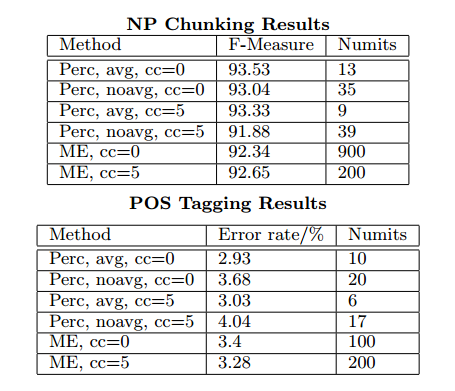
\includegraphics[width=9cm]{structperc}
  \end{center}
\end{frame}

\end{document}
